\documentclass[12pt]{article}

\usepackage[a5paper, landscape, margin=10mm]{geometry}
\usepackage{enumitem}
\usepackage{amsmath}
\usepackage{amssymb}
\usepackage{amsfonts}
\usepackage{placeins}
\usepackage{graphicx}
\usepackage{listings}
\usepackage{caption}
\usepackage{colortbl}
\usepackage[parfill]{parskip}
\usepackage[mathscr]{euscript}
\usepackage[usenames,dvipsnames,svgnames,table,hyperref]{xcolor}
\usepackage[hidelinks]{hyperref}
\usepackage{fontspec}
\usepackage{mdframed}

\setsansfont{FreeSans}
\setmonofont{Ubuntu Mono}
\renewcommand{\familydefault}{\sfdefault}

\hyphenation{WebGL}

\definecolor{webColor}{RGB}{0, 108, 174}
\newcommand{\web}[1]{{\color{webColor} \small \url{#1}}}
\newcommand{\webText}[2]{{\color{webColor} \href{#2}{#1}}}
\newcommand{\email}[2]{{\small \color{webColor} \textsf{\href{mailto:#1@#2}{#1[at]#2}}}}
\definecolor{titleColor}{RGB}{179, 0, 149}
\newcommand{\myTitle}[1]{{\large \color{titleColor} \hspace{-4mm} \textbf{\textsf{#1}}}}
\definecolor{subColor}{RGB}{179, 0, 149}
\newcommand{\mySub}[1]{\textsf{\color{subColor}#1}}
\definecolor{keyColor}{RGB}{170, 149, 0}
\newcommand{\myKey}[1]{\textbf{\color{keyColor}#1}}

\definecolor{redBoxFg}{RGB}{255, 0, 0}
\definecolor{redBoxBg}{RGB}{255, 218, 232}
\newcommand{\redBox}[1]{{\color{redBoxFg}\colorbox{redBoxBg}{#1}}}
\definecolor{yellowBoxFg}{RGB}{0, 0, 0}
\definecolor{yellowBoxBg}{RGB}{255, 232, 0}
\newcommand{\yellowBox}[1]{{\color{yellowBoxFg}\colorbox{yellowBoxBg}{#1}}}
\definecolor{greenBoxFg}{RGB}{0, 0, 0}
\definecolor{greenBoxBg}{RGB}{134, 210, 153}
\newcommand{\greenBox}[1]{{\color{greenBoxFg}\colorbox{greenBoxBg}{#1}}}
\definecolor{blueBoxFg}{RGB}{0, 0, 255}
\definecolor{blueBoxBg}{RGB}{218, 232, 255}
\newcommand{\blueBox}[1]{{\color{blueBoxFg}\colorbox{blueBoxBg}{#1}}}
\definecolor{violetBoxFg}{RGB}{0, 0, 0}
\definecolor{violetBoxBg}{RGB}{218, 204, 255}
\newcommand{\violetBox}[1]{{\color{violetBoxFg}\colorbox{violetBoxBg}{#1}}}

\mdfdefinestyle{MyFrame}{%
    linecolor=black,
    outerlinewidth=0pt,
    linewidth=0pt,
    innertopmargin=2.7pt,
    innerbottommargin=0pt,
    innerrightmargin=0pt,
    innerleftmargin=0pt,
        leftmargin = 0pt,
        rightmargin = 0pt}

\definecolor{lightttColor}{RGB}{69, 69, 80}
\newcommand{\lighttt}[1]{{\color{lightttColor}\texttt{#1}}}

\renewcommand*\labelenumi{(\theenumi)}
\renewcommand*{\theenumii}{\roman{enumii}}
\renewcommand*\labelenumii{\theenumii.}

\newcommand{\fixminipage}{\raggedright \setlength{\parskip}{0.3\baselineskip}}
\newcommand{\codeminipage}{\raggedright \setlength{\parskip}{0\baselineskip}}
\sloppy
\pagenumbering{gobble}


\begin{document}

\tikzstyle{smallnode} = [rectangle, minimum width=1.25cm, minimum height=1cm, text centered, text width=1.25cm, draw=black, fill=white]
\tikzstyle{smallishnode} = [rectangle, minimum width=2cm, minimum height=1cm, text centered, text width=2cm, draw=black, fill=white]
\tikzstyle{normalnode} = [rectangle, minimum width=3cm, minimum height=1cm, text centered, text width=3cm, draw=black, fill=white]
\tikzstyle{widenode} = [rectangle, minimum width=62mm, minimum height=8mm, text centered, text width=62mm, draw=black, fill=white]
\tikzstyle{bignode} = [rectangle, minimum width=3.5cm, minimum height=2cm, text centered, text width=3cm, draw=black, fill=white]
\tikzstyle{smemnode} = [rectangle, minimum width=3cm, minimum height=1cm, text centered, text width=3cm, draw=keyColorB, fill=white]
\tikzstyle{gmemnode} = [rectangle, minimum width=3cm, minimum height=1cm, text centered, text width=3cm, draw=keyColorA, fill=white]
\tikzstyle{smallishsmemnode} = [rectangle, minimum width=2cm, minimum height=1cm, text centered, text width=2cm, draw=keyColorB, fill=white]
\tikzstyle{arrow} = [thick,->,>=stealth]
\tikzstyle{line} = [thick]

\tikzstyle{rednode} = [normalnode, draw=redBoxFg, fill=redBoxBg, text=redBoxFg]
\tikzstyle{yellownode} = [normalnode, draw=yellowBoxFg, fill=yellowBoxBg, text=yellowBoxFg]
\tikzstyle{greennode} = [normalnode, draw=greenBoxFg, fill=greenBoxBg, text=greenBoxFg]
\tikzstyle{bluenode} = [normalnode, draw=blueBoxFg, fill=blueBoxBg, text=blueBoxFg]
\tikzstyle{violetnode} = [normalnode, draw=violetBoxFg, fill=violetBoxBg, text=violetBoxFg]

\tikzstyle{Mnode} = [greennode, text width=55mm, minimum width=55mm, minimum height=7mm]
\tikzstyle{Nnode} = [violetnode, text width=7mm, minimum width=7mm, minimum height=7mm]

\tikzstyle{producer} = [yellownode, text width=64mm, minimum width=64mm, minimum height=14mm]
\tikzstyle{consumer} = [greennode, text width=20mm, minimum width=20mm, minimum height=14mm]
\tikzstyle{smallproducer} = [yellownode, text width=20mm, minimum width=20mm, minimum height=14mm]
\tikzstyle{copylatency} = [rednode, text width=84mm, minimum width=84mm, minimum height=8mm]
\tikzstyle{ring} = [rednode, text width=16mm, minimum width=1mm, minimum height=14mm]
\newcommand{\consumerBox}[1]{{\color{greenBoxFg}\colorbox{greenBoxBg}{#1}}}
\newcommand{\producerBox}[1]{{\color{yellowBoxFg}\colorbox{yellowBoxBg}{#1}}}

{ \LARGE Exo Dev 2025-05-06 } \hfill { \LARGE \textbf{\textsf{Spork: GEMM Samples}}}

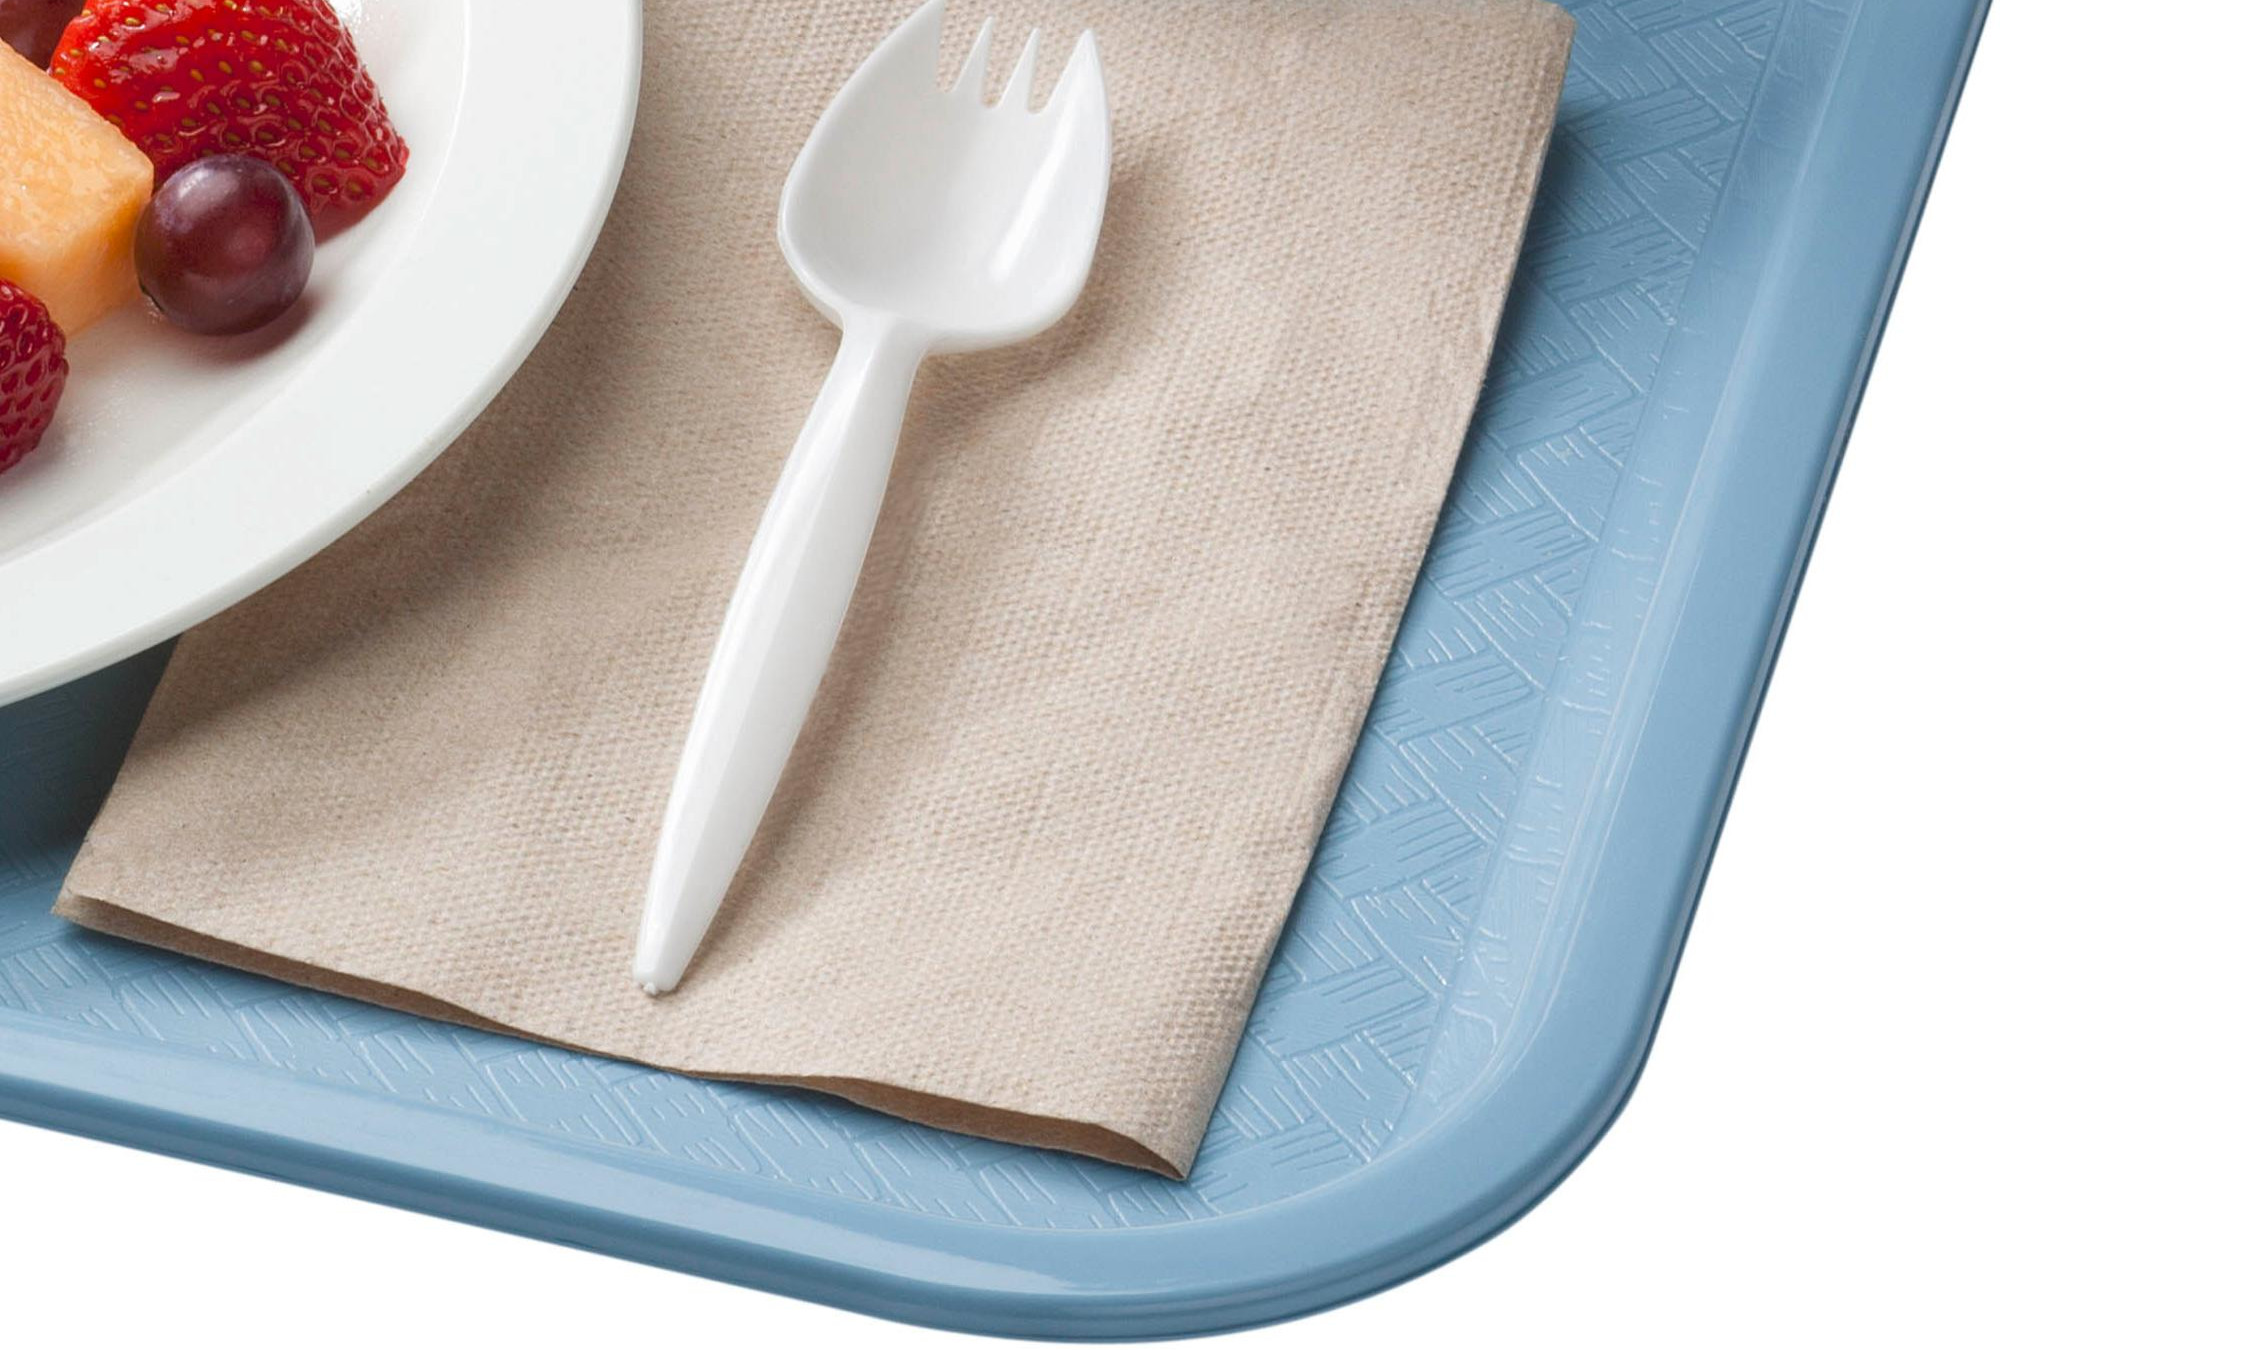
\includegraphics[width=\linewidth]{usda_spork.jpg}

\newpage
\myTitle{Intro 0}

\input{gemms_tex/intro.0.tex}
\newpage
\myTitle{Intro 1}

\input{gemms_tex/intro.1.tex}

\newpage
\myTitle{Intro 2}

\input{gemms_tex/intro.2.tex}

\newpage
\myTitle{Par}

\input{gemms_tex/par.0.tex}

\begin{tikzpicture}[node distance=2mm]
\node (cta) [yellownode, minimum width=30mm, minimum height=40mm] {CTA: 256 threads};

\node (m2) [Mnode, right=of cta, xshift=16mm] {\texttt{m1 = 2}; threads [32, 47]};
\node (m1) [Mnode, above=of m2] {\texttt{m1 = 1}; threads [16, 31]};
\node (m0) [Mnode, above=of m1] {\texttt{m1 = 0}; threads [0, 15]};
\node (m15) [Mnode, below=of m2, yshift=-9mm] {\texttt{m1 = 15}; threads [240, 255]};
\draw [arrow] (cta) -- node[above] {\texttt{for \redBox{m1}}} (m2);
\draw [dotted] (m2) -- (m15);
\node (m0n0) [Nnode, right=of m0, xshift=16mm] {0};
\node (m0n1) [Nnode, right=of m0n0] {1};
\node (m0n2) [Nnode, right=of m0n1] {2};
\node (m0n15) [Nnode, right=of m0n2, xshift=8mm] {15};
\node (m1n0) [Nnode, below=of m0n0] {16};
\node (m1n1) [Nnode, below=of m0n1] {17};
\node (m1n2) [Nnode, below=of m0n2] {18};
\node (m1n15) [Nnode, below=of m0n15] {31};
\node (m2n0) [Nnode, below=of m1n0] {32};
\node (m2n1) [Nnode, below=of m1n1] {33};
\node (m2n2) [Nnode, below=of m1n2] {34};
\node (m2n15) [Nnode, below=of m1n15] {47};
\node (m15n0) [Nnode, right=of m15, xshift=16mm] {240};
\node (m15n1) [Nnode, right=of m15n0] {241};
\node (m15n2) [Nnode, right=of m15n1] {242};
\node (m15n15) [Nnode, right=of m15n2, xshift=8mm] {255};
\draw [arrow] (m0) -- node[above] {\texttt{for \blueBox{n1}}} (m0n0);
\draw [arrow] (m1) -- node[above] {\texttt{for \blueBox{n1}}} (m1n0);
\draw [arrow] (m2) -- node[above] {\texttt{for \blueBox{n1}}} (m2n0);
\draw [arrow] (m15) -- node[below] {\texttt{for \blueBox{n1}}} (m15n0);
\draw [dotted] (m2n0) -- node[] {\texttt{n1 = 0}} (m15n0);
\draw [dotted] (m2n1) -- (m15n1);
\draw [dotted] (m2n2) -- node[] {\texttt{n1 = 2}} (m15n2);
\draw [dotted] (m2n15) --node[] {\texttt{n1 = 15}} (m15n15);
\draw [dotted] (m0n2) -- (m0n15);
\draw [dotted] (m1n2) -- (m1n15);
\draw [dotted] (m2n2) -- (m2n15);
\draw [dotted] (m15n2) -- (m15n15);

\end{tikzpicture}

\newpage
\myTitle{Tile 0}

\input{gemms_tex/tile.0.tex}
\newpage
\myTitle{Tile 1}

\input{gemms_tex/tile.1.tex}

\newpage
\myTitle{Tile 2}

\input{gemms_tex/tile.2.tex}

\newpage
\myTitle{GMEM}

\input{gemms_tex/gmem_remark.0.tex}

\newpage
\myTitle{SMEM Alloc}

\input{gemms_tex/smem_alloc.0.tex}

\newpage
\myTitle{Broken SMEM 0}

\input{gemms_tex/broken_smem.0.tex}

\newpage
\myTitle{Broken SMEM 1}

\input{gemms_tex/broken_smem.1.tex}

\newpage
\myTitle{Broken SMEM 2}

\input{gemms_tex/broken_smem.2.tex}

\newpage
\myTitle{Distributed Memory 0}

\input{gemms_tex/dmem.0.tex}

\newpage
\myTitle{Distributed Memory 1}

\input{gemms_tex/dmem.1.tex}

\newpage
\myTitle{Distributed Memory 2}

\input{gemms_tex/dmem.2.tex}

\newpage
\myTitle{Distributed Memory 3}

\input{gemms_tex/dmem.3.tex}

\newpage
\myTitle{Distributed Memory 4}

\input{gemms_tex/dmem.4.tex}
\newpage
\myTitle{Distributed Memory 5}

\begin{minipage}[t]{0.48\textwidth}\fixminipage
\mySub{Before}

\input{gemms_tex/dmem_before.0.tex}
\end{minipage}
\hfill
\begin{minipage}[t]{0.48\textwidth}\fixminipage
\mySub{After}

\input{gemms_tex/dmem_after.0.tex}

\vspace{4mm}
Distributed dimensions (\blacktt{f32[\greenBox{16}, \violetBox{16}, ...]}) are elided in the generated C++ code.
\end{minipage}

\newpage
\myTitle{Working SMEM Example 0}

\input{gemms_tex/working_smem.0.tex}

\newpage
\myTitle{Working SMEM Example 1}

\input{gemms_tex/working_smem.1.tex}
\newpage
\myTitle{Working SMEM Example 2}

\input{gemms_tex/working_smem.2.tex}

\newpage
\myTitle{Ring Buffer -- Why}

Hardware underutilized -- strictly separate memory (``produce'': load SMEM) and compute (``consume'': accumulate) workloads.

\begin{tikzpicture}[node distance=2mm]
\node (produce0) [producer] {Produce \texttt{k1 = 0}};
\node (consume0) [consumer, right=of produce0] {Consume \texttt{k1 = 0}};
\node (produce1) [producer, right=of consume0] {Produce \texttt{k1 = 1}};
\node (consume1) [consumer, right=of produce1] {Consume \texttt{k1 = 1}};
\end{tikzpicture}

Overlap produce and consume workloads

\begin{tikzpicture}[node distance=2mm]
\node (produce0) [producer] {Produce \texttt{k1 = 0}};
\node (consume0) [consumer, right=of produce0] {Consume \texttt{k1 = 0}};
\node (produce1) [producer, below=of produce0, xshift=24mm] {Produce \texttt{k1 = 1}};
\node (consume1) [consumer, right=of produce1] {Consume \texttt{k1 = 1}};
\node (produce2) [producer, below=of produce1, xshift=24mm] {Produce \texttt{k1 = 2}};
\node (consume2) [consumer, right=of produce2] {Consume \texttt{k1 = 2}};
\node (produce3) [producer, below=of produce2, xshift=24mm] {Produce \texttt{k1 = 3}};
\node (consume3) [consumer, right=of produce3] {Consume \texttt{k1 = 3}};
\node (produce4) [producer, below=of produce3, xshift=24mm] {Produce \texttt{k1 = 4}};
\node (consume4) [consumer, right=of produce4] {Consume \texttt{k1 = 4}};
\end{tikzpicture}

\newpage
\myTitle{Ring Buffer -- Why}

Latency of \producerBox{producer} (memory) workloads is very long compared to \consumerBox{consumer} workloads.

We need a deep ring buffer to hide latency.
Many copies are in flight simultaneously.

\begin{tikzpicture}[node distance=2mm]
\node (produce0) [producer] {Produce \texttt{k1 = 0}};
\node (consume0) [consumer, right=of produce0] {Consume \texttt{k1 = 0}};
\node (produce1) [producer, below=of produce0, xshift=24mm] {Produce \texttt{k1 = 1}};
\node (consume1) [consumer, right=of produce1] {Consume \texttt{k1 = 1}};
\node (produce2) [producer, below=of produce1, xshift=24mm] {Produce \texttt{k1 = 2}};
\node (consume2) [consumer, right=of produce2] {Consume \texttt{k1 = 2}};
\node (produce3) [producer, below=of produce2, xshift=24mm] {Produce \texttt{k1 = 3}};
\node (consume3) [consumer, right=of produce3] {Consume \texttt{k1 = 3}};
\node (produce4) [producer, right=of consume0] {Produce \texttt{k1 = 4}};
\node (consume4) [consumer, right=of produce4] {Consume \texttt{k1 = 4}};
\node (produce5) [producer, right=of consume1] {Produce \texttt{k1 = 5}};
\node (consume5) [consumer, right=of produce5] {Consume \texttt{k1 = 5}};
\node (produce6) [producer, right=of consume2] {Produce \texttt{k1 = 6}};
\node (produce7) [producer, right=of consume3] {Produce \texttt{k1 = 7}};
\node (ring0) [ring, left=of produce0] {Buffer 0};
\node (ring1) [ring, below=of ring0] {Buffer 1};
\node (ring2) [ring, below=of ring1] {Buffer 2};
\node (ring3) [ring, below=of ring2] {Buffer 3};
\draw [arrow] (produce0) to[out=45, in=135] node [above] (forward) {\violetBox{Arrive/Await}} (consume0);
\draw [arrow] (consume0) to[out=45, in=135] node [above] (forward) {\violetBox{ReverseArrive/ReverseAwait}} (produce4);
\end{tikzpicture}

Forward synchronization: Consumer \consumerBox{\texttt{k1 = N}} waits for producer \producerBox{\texttt{k1 = N}}\\
(RAW hazard: we need to wait for the SMEM tiles to be filled)

Reverse synchronization: Producer \producerBox{\texttt{k1 = N}} waits for consumer \consumerBox{\texttt{k1 = N - 4}}\\
(WAR hazard: we need to not overwrite SMEM tiles before they're fully consumed)

\newpage
\myTitle{Warp Specialization}

Dedicate some warps (32-thread groups) to be \producerBox{producers} and some to be \consumerBox{consumers}.

\begin{tikzpicture}[node distance=2mm]
\node (produce0) [smallproducer] {Copy instr \texttt{k1 = 0}};
\node (produce1) [smallproducer, right=of produce0] {Copy instr \texttt{k1 = 1}};
\node (produce2) [smallproducer, right=of produce1] {Copy instr \texttt{k1 = 2}};
\node (produce3) [smallproducer, right=of produce2] {Copy instr \texttt{k1 = 3}};
\node (produce4) [smallproducer, right=of produce3] {Copy instr \texttt{k1 = 4}};
\node (produce5) [smallproducer, right=of produce4] {Copy instr \texttt{k1 = 5}};
\node (produce6) [smallproducer, right=of produce5] {Copy instr \texttt{k1 = 6}};
\node (produce7) [smallproducer, right=of produce6] {Copy instr \texttt{k1 = 7}};
\node (producers) [text width=19mm, left=of produce0] {Threads [256, 383]};
\node (copy0) [copylatency, below=of produce0, xshift=32mm] {Copy latency (to buffer 0)};
\node (copy1) [copylatency, below=of copy0, xshift=25mm] {Copy latency (to buffer 1)};
\node (copy2) [copylatency, below=of copy1, xshift=25mm] {Copy latency (to buffer 2)};
\node (copy3) [copylatency, below=of copy2, xshift=25mm] {Copy latency (to buffer 3)};
\node (copy4) [copylatency, right=of copy0, xshift=11mm] {Copy latency (to buffer 0)};
\node (copy5) [copylatency, below=of copy4, xshift=25mm] {Copy latency (to buffer 1)};
\node (copy6) [copylatency, below=of copy5, xshift=25mm] {Copy latency (to buffer 2)};
\node (copy7) [copylatency, below=of copy6, xshift=25mm] {Copy latency (to buffer 3)};
\node (consume0) [consumer, below=of copy3, xshift=-18mm] {Consume \texttt{k1 = 0}};
\node (consume1) [consumer, right=of consume0] {Consume \texttt{k1 = 1}};
\node (consume2) [consumer, right=of consume1] {Consume \texttt{k1 = 2}};
\node (consume3) [consumer, right=of consume2] {Consume \texttt{k1 = 3}};
\node (consume4) [consumer, right=of consume3] {Consume \texttt{k1 = 4}};
\node (consumer) [text width=19mm, left=of consume0] {Threads [0, 255]};

%% \draw[arrow, dotted] (produce0.south) to[out=270, in=135] (copy0.west);
%% \draw[arrow, dotted] (produce1.south) to[out=270, in=135] (copy1.west);
%% \draw[arrow, dotted] (produce2.south) to[out=270, in=135] (copy2.west);
%% \draw[arrow, dotted] (produce3.south) to[out=270, in=135] (copy3.west);
%% \draw[arrow, dotted] (produce4.south) to[out=270, in=135] (copy4.west);
%% \draw[arrow, dotted] (produce5.south) to[out=270, in=135] (copy5.west);
%% \draw[arrow, dotted] (produce6.south) to[out=270, in=135] (copy6.west);
%% \draw[arrow, dotted] (produce7.south) to[out=270, in=135] (copy7.west);

\draw[arrow, dotted] (copy0.east) to[out=315, in=90] (consume0.north);
\draw[arrow, dotted] (copy1.east) to[out=315, in=90] (consume1.north);
\draw[arrow, dotted] (copy2.east) to[out=315, in=90] (consume2.north);
\draw[arrow, dotted] (copy3.east) to[out=315, in=90] (consume3.north);
\end{tikzpicture}

\newpage
\myTitle{Ring Buffer 0}

\input{gemms_tex/ring.0.tex}

\newpage
\myTitle{Ring Buffer 1}

\input{gemms_tex/ring.1.tex}

\newpage
\myTitle{Ring Buffer 2}

\input{gemms_tex/ring.2.tex}

\newpage
\myTitle{Problem With Copies}

\input{gemms_tex/sync_copy.0.tex}

\newpage
\myTitle{TMA (Bulk Copy) Instructions}

\begin{minipage}[t]{0.48\textwidth}\fixminipage
\begin{itemize}
\item A single \texttt{cp.bulk.async} instruction can copy a large 1D-5D tile \myKey{GMEM}$\leftrightarrow$\myKeyB{SMEM}
\item \myKeyB{SMEM} tile: densely packed C-order matrix
\begin{itemize}
  \item 128 byte alignment
\end{itemize}
\item \myKey{GMEM} tile: tile from big C-order matrix
\begin{itemize}
  \item \myKey{Predicated} and strided
  \item 16 byte aligned memory and strides
\end{itemize}
\end{itemize}

\begin{tikzpicture}[node distance=5mm]
\node (smem) [smemnode] {\myKeyB{SMEM tile}};
\node (gmembig) [bignode, right=of smem, yshift=-3mm] {};
\node (gmem) [gmemnode, right=of smem, xshift=9mm] {\myKey{GMEM tile}};
\draw [arrow] ($(smem.east)-(0,0.2)$) -- ($(gmem.west)-(0,0.2)$);
\draw [arrow] ($(gmem.west)+(0,0.2)$) -- ($(smem.east)+(0,0.2)$);
\end{tikzpicture}
\end{minipage}
\hfill
\begin{minipage}[t]{0.48\textwidth}\fixminipage
\mySub{Contrast with synchronous copy instructions}
\begin{itemize}
  \item Copies large tiles instead of only 4/8/16 bytes at a time.
  \item Bypasses registers
  \item Async copy: execution continues \textit{without waiting for copy to finish}
  \item Async copies don't interact with normal synchronization, e.g. \texttt{\_\_syncthreads();}
\end{itemize}

\mySub{Actor Kind}

Exo-GPU will categorize instructions based on \myKeyA{actor kind}; essentially, instructions that operate on different timelines have different actor kinds.
\begin{itemize}
  \item \texttt{cpu}: CPU instructions
  \item \texttt{cuda\_classic}: CUDA non-async instr
  \item \texttt{tma\_to\_smem\_async}: async copies to SMEM
  \item \texttt{wgmma\_async}: Async H100 tensor core
  \item ...
\end{itemize}
Parameterize sync statements (Fence/Arrive/Await) with \myKeyA{actor kind}; lowers to barriers that target a specific instruction category.
\end{minipage}

\newpage
\myTitle{Before TMA}

\input{gemms_tex/ring.3.tex}

\newpage
\myTitle{Prep TMA 0}

\input{gemms_tex/prep_tma.0.tex}

\newpage
\myTitle{Prep TMA 1}

\input{gemms_tex/prep_tma.1.tex}

\newpage
\myTitle{TMA 0}

\input{gemms_tex/tma.0.tex}

\newpage
\myTitle{TMA 1}

\input{gemms_tex/tma.1.tex}

\newpage
\myTitle{TMA 2}

\input{gemms_tex/tma.2.tex}

\newpage
\myTitle{TMA 3}

\input{gemms_tex/tma.3.tex}

\newpage
\myTitle{TMA Forward Synchronization}

\input{gemms_tex/prep_tma.2.tex}

\newpage
\myTitle{TMA Reverse Synchronization}

\input{gemms_tex/prep_tma.3.tex}

\newpage
\myTitle{Next Steps: Tensor Cores}

\input{gemms_tex/wgmma.0.tex}


\end{document}
